\documentclass[10pt,a4paper]{article}
% The following LaTeX packages must be installed on your machine: amsmath, authblk, bm, booktabs, caption, dcolumn, fancyhdr, geometry, graphicx, hyperref, latexsym, natbib
\input{192.dat}
\usepackage{gensymb}
\usepackage{float}
\usepackage{siunitx}
\usepackage{amssymb}
\usepackage{float}
\usepackage{listings}
\PassOptionsToPackage{hyphens}{url}\usepackage{hyperref}
\usepackage[none]{hyphenat}
%\renewcommand{\familydefault}{\sfdefault}


\begin{document}

\setcounter{page}{1}

\section*{Exam 1: Results and Discussion}

\begin{table}
	\centering
	\caption{Summary of descriptive statistics of the given data.}
	\begin{tabular}{c|ccccccccc}
Variable & N & N*	& Mean	& SE Mean	& StDev	& Minimum	& Q1	& Median	& Q3 \\ \hline \hline
Turn Diameter	& 109	& 0	& 35.514	& 0.318	& 3.321	& 28.200	& 32.800	& 35.400	& 38.100 \\
Horsepower	& 109	& 0	& 124.67	& 3.85	& 40.16	& 55.00	& 93.00	& 114.00	& 155.00 \\
Number of miles per gallon	& 109	& 0	& 21.486	& 0.375	& 3.917	& 14.000	& 18.000	& 21.000	& 24.000
	\end{tabular}
	\label{tab:summary}
\end{table}

\begin{figure}[tb]
	\centering
	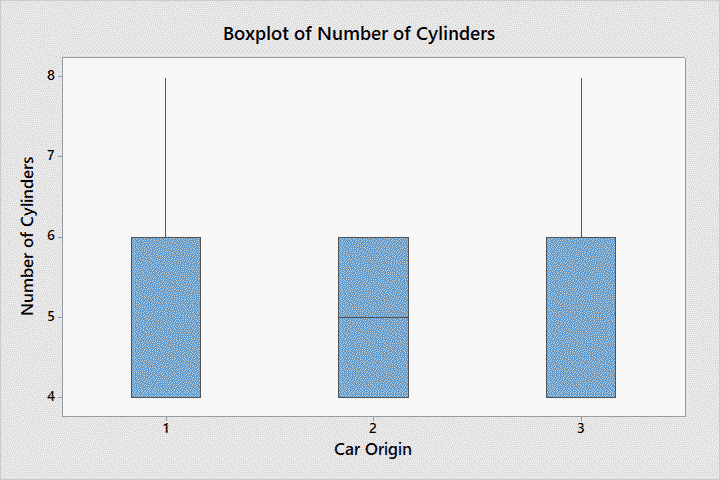
\includegraphics[width=0.75\linewidth]{box-cyl_vs_orig.png}
	\caption{}
	\label{fig:cyl-vs-orig}
\end{figure}

Figure \ref{fig:cyl-vs-orig} shows a boxplot of the number of cylinders produced by each car manufacturer. It shows that Car Origin 1 and 3 manufacture a variety of vehicles having 4-- to 8--cylinder engines, while Car Origin 2 only manufactures 4-- to 6--cylinder engines. The plot also shows that all three manufacturers tend to favor production of more cars equipped with 4-- to 6--cylinder engines.

\begin{figure}[tb]
	\centering
	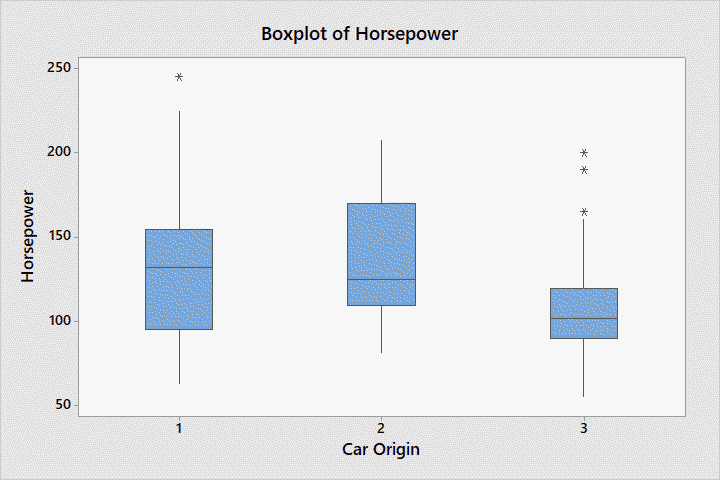
\includegraphics[width=0.75\linewidth]{box-hp_vs_orig.png}
	\caption{}
	\label{fig:hp-vs-orig}
\end{figure}

Figure \ref{fig:hp-vs-orig} shows a boxplot of horsepower (HP) vs the car origin. Car Origins 1 and 2 produce vehicles with roughly the same HP range. Among the data, Car Origin 1 has one outlier just below 250 HP. Car Origin 2, while producing similar HP range as Car Origin 1, has a median below that of the latter. Car Origin 3 produces vehicles with a much tighter range and below that of either Car Origin 1 and 2, while having three outliers above the fourth quartile.

\begin{figure}[tb]
	\centering
	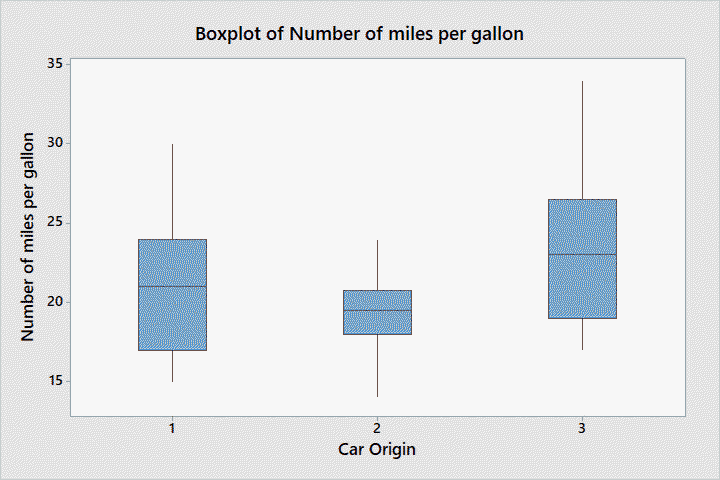
\includegraphics[width=0.75\linewidth]{box-mpg_vs_orig.png}
	\caption{}
	\label{fig:mpg-vs-orig}
\end{figure}

Figure \ref{fig:mpg-vs-orig} shows the miles per gallon (MPG) for each car manufacturer. Car Origin 3 produces vehicles with the best fuel economy, as its median is higher than that of either Car Origin 1 and 2. The latter has a more controlled range of fuel economy but also has the most inefficient. Car Origin 1 sits between the other two and has a range of MPG similar to Car Origin 3.

\begin{figure}[tb]
	\centering
	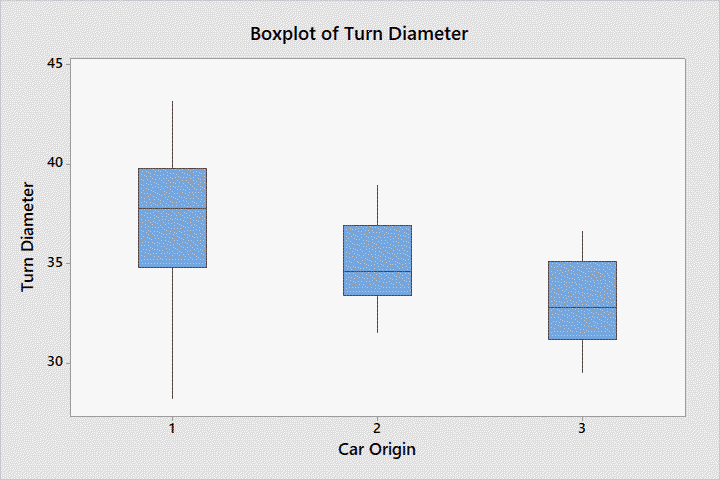
\includegraphics[width=0.75\linewidth]{box-td_vs_orig.png}
	\caption{}
	\label{fig:td-vs-orig}
\end{figure}

Figure \ref{fig:td-vs-orig} shows the turn diameters for each car manufacturer. At first glance, the inverse proportionality is evident. Car Origin 1 produces vehicles with the highest turn diameters, but also has the widest range. Car Origin 2 and 3 produce a roughly similar range, with the former sitting between the other two.

\begin{figure}[tb]
	\centering
	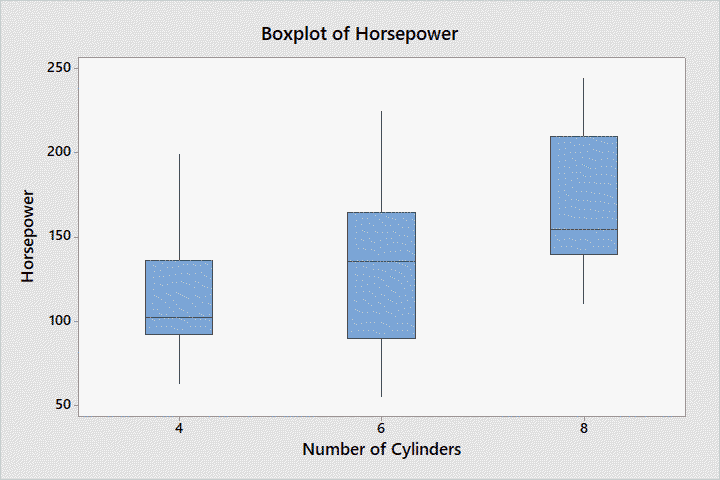
\includegraphics[width=0.75\linewidth]{box-hp_vs_cyl.png}
	\caption{}
	\label{fig:hp-vs-cyl}
\end{figure}

Figure \ref{fig:hp-vs-cyl} shows the HP vs the number of cylinders. As one would expect, more engine cylinders would cause more displacement and subsequently, more horsepower. 

\begin{figure}[tb]
	\centering
	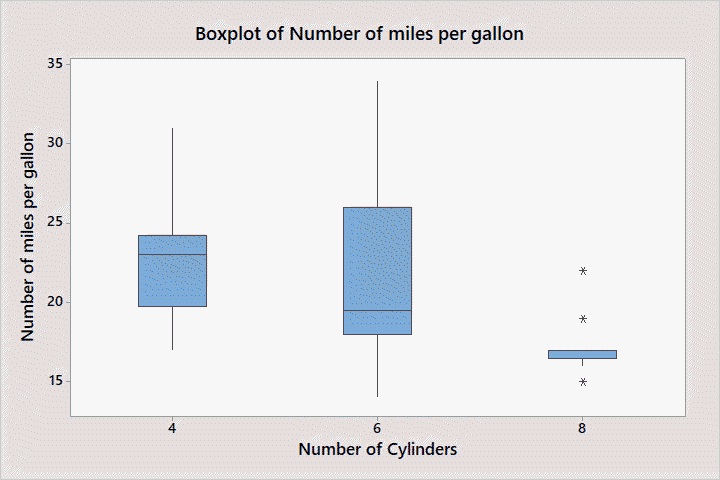
\includegraphics[width=0.75\linewidth]{box-mpg_vs_cyl.png}
	\caption{}
	\label{fig:mpg-vs-cyl}
\end{figure}

Figure \ref{fig:mpg-vs-cyl} shows the MPG for each number of cylinders. A 4--cylinder engine shows moderate fuel economy, while a 6--cylinder setup varies more widely. An 8--cylinder engine tends to be consistent in having the worst fuel economy, with two outliers above the 4th quartile, while still below the median of a 4--cylinder engine. It also has one outlier below the 1st quartile.

\begin{figure}[tb]
	\centering
	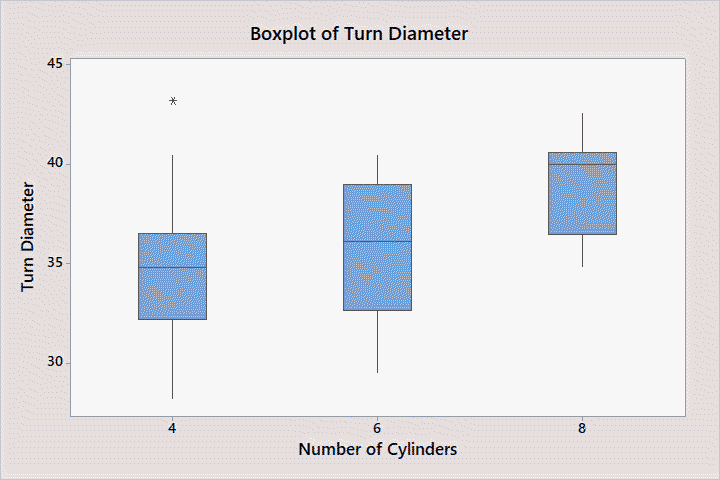
\includegraphics[width=0.75\linewidth]{box-td_vs_cyl.png}
	\caption{}
	\label{fig:td-vs-cyl}
\end{figure}

Figure \ref{fig:td-vs-cyl} shows the relation of turn diameter with the number of cylinders. On initial inspection, it is evident that the turn diameter generally increases with the number of engine cylinders. The 4--cylinder setup has one outlier above the 4th quartile which is higher than the median of the 8--cylinder setup.

\begin{figure}[tb]
	\centering
	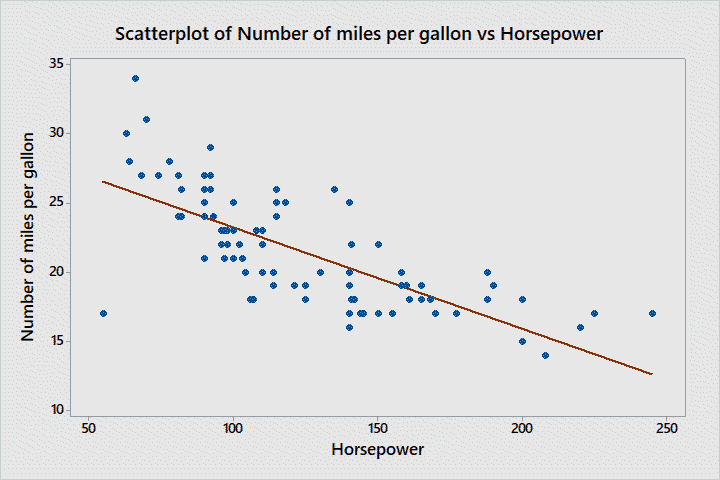
\includegraphics[width=0.75\linewidth]{mpg_vs_hp.png}
	\caption{}
	\label{fig:scatter-mpg-vs-hp}
\end{figure}

Figure \ref{fig:scatter-mpg-vs-hp} shows a scatter plot of number of MPG vs HP. The regression line has a Pearson correlation of $-0.755$ and a $p$-value of $< 0.05$, indicating strong correlation between MPG and HP.

\end{document}